\section{Disclaimer}
\begin{itemize}
    \item El laboratorio 06 es una leve modificacion al laboratorio 05
    \item Siguiendo la instruccion de poder reutilizar codigo de otros laboratorios, el trabajo practicamente esta hecho en un 70%, aqui mostraremos las modificaciones partiendo de base en el laboratorio 05
    \item Para seguir el historial de modificaciones, utilizaremos los commits como referencia
    \item Los commits fueron hechos con el enfoque de las 7 reglas de los buenos commits (La convencion que sugiere el mismo git), que consta de un titulo y un cuerpo
    \item El titulo contiene, en forma imperativa, la accion que se llevara a cabo en cada uno de los commits, esta en modo imperativo para responder a la pregunta "Este commit, si se aplica, hace.." 
    \item El body contiene detalles sobre los cambios introducidos en el commit
    \item Dada la naturaleza de los commit como reportes, el presente informe de laboratorio se podra detallar completamente con los mensajes del body, agregare comentarios unicamente donde sean pertinentes
\end{itemize}
\section{Cambiando modelo a ArrayList}
\begin{itemize}
    \item La primera modificacion viene sobre el uso de arrays bidimensaionales, para cambiarlo a usar ArrayList bidimensionales, para esto tendremos que tomar en cuenta la forma de introducir y obtener datos de un ArrayList
\end{itemize}

\begin{lstlisting}[language=bash, caption={Commit principal}]
commit 394799acf85f7bbde78257b4c2deb3d9a90b6674
Author: JhonatanDczel <jariasq@unsa.edu.pe>
Date:   Mon Oct 16 15:58:14 2023 -0500

    Lab 06: Cambiando modelo a ArrayList

    Dado que la unica expecificaciones que el tablero sea un arraylist, es
    unt rabajo trivial cambiar de tipo de lista y cambiar tambien la forma
    en que se accede a los elementos y como se setean elementos
\end{lstlisting}
\begin{itemize}
    \item El principal cambio que se hizo, fue declarar board como un array list bidimensaional de tamanho 10, luego se recorre el ArrayList para crear otros 10 ArrayList dentro de ellos, generando asi las filas y columnas
\end{itemize}
\begin{lstlisting}[language=java, caption={VideoJuego.java}]
  public static ArrayList<ArrayList<Soldado>> board = new ArrayList<>(10);
  public static Picture gBoard;
  public static Soldado maxLife = new Soldado("sold");
  public static int promedio = 0;
  
  public static void main(String[] args){
    for (int i = 0; i < 10; i++) {
      ArrayList<Soldado> fila = new ArrayList<>(10);
      for (int j = 0; j < 10; j++) {
        fila.add(null);
      }
      board.add(fila);
    }
\end{lstlisting}

\section{Creando dos ejercitos}
\begin{lstlisting}[language=bash, caption={Commit principal}]
commit d4c878a641ecad05ce16390458da3bf0d0018fd3
Author: JhonatanDczel <jariasq@unsa.edu.pe>
Date:   Mon Oct 16 16:02:24 2023 -0500

    Crea dos ejercitos de soldados y los muestra

    Se crean dos ejercitos, seteando sus nombres con "1x1"... luego se
    ubican en pantalla y los datos de creacion se muestran por consola
\end{lstlisting}
\begin{itemize}
    \item Los cambios se veran a continuacion:
\end{itemize}
\begin{lstlisting}[language=java, caption={VideoJuego.java}]
    Soldado[] army1 = initializeArmy(1); 
    Soldado[] army2 = initializeArmy(2); 

    displayArmy(army1);
    displayArmy(army2);
...
...
...
  public static Soldado[] initializeArmy(int n){
    int promLife = 0;
    Random rand = new Random();
    int randNum = rand.nextInt(10) + 1;
    Soldado[] army = new Soldado[randNum];

    for(int i = 0; i < randNum; i++){
      army[i] = new Soldado("Soldado " + n + "x" + (i + 1));
      army[i].setLife(rand.nextInt(5) + 1);
      if(army[i].getLife() > maxLife.getLife())
        maxLife = army[i];
      promLife += army[i].getLife();
      genColumnRow(army[i]);
    }
    promLife = promLife / army.length;
    promedio = (promLife + promedio) / 2;
    return army;
  }

\end{lstlisting}
\begin{itemize}
    \item El cambio fue en la manera en que se agregan los nombres, para adecuarlos a 1x0.. 1x2...
\end{itemize}
\section{Ranking de soldados por vida}

\begin{lstlisting}[language=bash, caption={Commit principal}]
commit 6316d6416b04735eefb840dc9898c7be70712a4c
Author: JhonatanDczel <jariasq@unsa.edu.pe>
Date:   Mon Oct 16 16:11:06 2023 -0500

    Agregar ranking de soldados por vida

    Se agrego la funcionalidad de hacer un ranking de soldados, para eso, se
    juntan los dos ejercitos y luego se aplica el ordenamiento por bubble
    sort
\end{lstlisting}
\begin{itemize}
    \item El ranking se hizo usando bubble sort como algoritmo de ordenamiento
    \item El segundo algoritmo de ordenamiento que se utiliza es insertion sort
    \item Como tenemos dos ejercitos, se crea un nuevo array uniendo a los dos, y luego se aplica el ordenamiento
\end{itemize}
\begin{lstlisting}[language=java, caption={VideoJuego.java}]
  public static void insertionSortLife(Soldado[] army){
    for(int i = 1; i < army.length; i++){
      Soldado actual = army[i];
      int j = i - 1;
      while(j >= 0 && army[j].getLife() > actual.getLife()){
        army[j + 1] = army[j];
        j--;
      }
      army[j + 1] = actual;
    }
  }

  public static void bubbleSortLife(Soldado[] army){
    for(int i = 0; i < army.length - i; i++){
      for(int j = 0; j < army.length - 1 - i; j++){
        if(army[j].getLife() > army[j + 1].getLife())
          intercambiar(army, j, j + 1);
      }
    }
  }
  public static void intercambiar(Soldado[] army, int i, int j){
    Soldado aux = army[i];
    army[i] = army[j];
    army[j] = aux;
  }
}
\end{lstlisting}
\begin{itemize}
    \item Se usan 3 metodos, uno auxiliar para intercambiar, y otros dos que son Bubble e Insertion sort
\end{itemize}
\section{Implementar forma de encontrar un ganador}
\begin{lstlisting}[language=bash, caption={Commit principal}]
commit bad9e0d93b8adc82891638530b51dc0250daa7d1
Author: JhonatanDczel <jariasq@unsa.edu.pe>
Date:   Mon Oct 16 16:17:23 2023 -0500

    Implementa mecanismo para determinar ganador

    Se implemento el metodo WhoWins, que detecta cual de los dos ejercitos
    resulto como ganador, para esto se basa en la cantidad de soldados que
    tiene cada ejercito, ya que siempre se impondra la cantidad numerica en
    una batalla
\end{lstlisting}
\begin{itemize}
    \item Como ya esta mencionado, la forma de encontrar un ganador es comparando la cantidad nunmerica de soldados
\end{itemize}

\section{Adicional: Distintos colores, distintos ejercitos}
\begin{itemize}
    \item Para aplicar un atractivo visual, y para distinguir entre ejercitos, vamos a implementar en el codigo la funcionalidad de especificar si queremos que un ejercito sea de color negro
\end{itemize}
\begin{lstlisting}[language=bash, caption={Commit principal}]
commit 4b5eecad1cf099cf55b1e66815fc5c8cf952848c (HEAD -> main, origin/main)
Author: JhonatanDczel <jariasq@unsa.edu.pe>
Date:   Mon Oct 16 16:43:16 2023 -0500

    Implementacion de distinto color para ejercitos

    Se agrego una moficiacion en Videojuego.java, para pintar de negro
    ciertos ejercitos y asi tener dos colores para representarlos
    El Soldado.java se agrego un nuevo atributo, que indica si un soldado
    debera colorearse de negro o no
\end{lstlisting}
\begin{itemize}
    \item Para eso primero se modifica la clase soldado
    \item Agregamos un nuevo atributo
    \item Agregamos metodos getters
    \item Agregamos metodos setters
\end{itemize}
\begin{lstlisting}[language=java, caption={Soldado.java}]
public class Soldado{
...
...
  public boolean negro = false;

  public Soldado(String name){
    this.name = name;
  }

  //SECCION DE SETERS

  public void setNegro(boolean n){
    this.negro = n;
 ...
 ...
 
  //SECCION DE GETERS

...
...

  public boolean getNegro(){
    return this.negro;
  }
  
...
...

}
\end{lstlisting}
\begin{itemize}
    \item Ahora se agrega una sentencia if a nuestro metodo makeGBoard, que genera el tablero grafico
\end{itemize}
\begin{lstlisting}[language=java, caption={Soldado.java}]
...
...

        Picture c = Picture.casilleroBlanco();
        if(board.get(i).get(j) != null){
          Picture sold = Picture.soldier();
          if(board.get(i).get(j).getNegro())
            sold = sold.invertir();
          c = sold.superponer(c);
        }

...
...
\end{lstlisting}
\begin{itemize}
    \item Con esta condicional, en caso de que el atributo negro de Soldado.java sea true, se invertira el color del soldado
    \item Para invertir el color, se usa el metodo de la clase Picture, en la biblioteca graphics
\end{itemize}

\section{Ejecucion}
\begin{itemize}
    \item A continuacion veremos un ejemplo de la simulacion de batalla
    \item Tenemos dos salidas, una grafica y otra por consola
    \item La grafica por consola muestra:
    \begin{itemize}
        \item Los datos de los soldados de los ejercitos creados
        \item Los datos del soldado con mas puntos
        \item El ranking de soldados tomando como referencia la cantidad de vida que poesen
        \item El ganador de la batalla tomando en cuenta el factor de la cantidad numerica de soldados en ambos ejercitos
    \end{itemize}
    \item La grafica del campo de batalla contiene a los soldados que han sido creados, cada uno ubicado en su posicion en filas y columnas
\end{itemize}
\subsection{Grafica del campo}

\centering
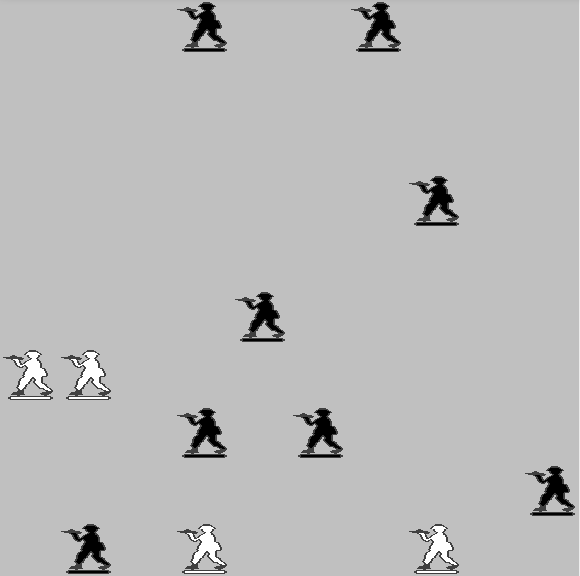
\includegraphics[width=0.5\textwidth]{img/campo-de-batalla.png}
\begin{itemize}
    \item Cada soldado corresponde a uno que ha sido creado, y esta ubicado en la misma posicion que lo que indica la consola
\end{itemize}

\subsection{Grafica por consola}
\begin{itemize}
    \item A continuacion veremos la salida de consola:
\end{itemize}

\begin{lstlisting}[language=bash, caption={Ejecucion por consola}]
===== Ejercito 1 =====
 Soldado 1x1:
  Nivel de vida: 2
  Fila: 1
  Columna: 7

 Soldado 1x2:
  Nivel de vida: 4
  Fila: 1
  Columna: 4

 Soldado 1x3:
  Nivel de vida: 2
  Fila: 4
  Columna: 8

 Soldado 1x4:
  Nivel de vida: 5
  Fila: 8
  Columna: 4

 Soldado 1x5:
  Nivel de vida: 1
  Fila: 6
  Columna: 5

 Soldado 1x6:
  Nivel de vida: 3
  Fila: 10
  Columna: 2

 Soldado 1x7:
  Nivel de vida: 1
  Fila: 8
  Columna: 6

 Soldado 1x8:
  Nivel de vida: 1
  Fila: 9
  Columna: 10


===== Ejercito 2 =====
 Soldado 2x1:
  Nivel de vida: 3
  Fila: 10
  Columna: 4

 Soldado 2x2:
  Nivel de vida: 2
  Fila: 7
  Columna: 2

 Soldado 2x3:
  Nivel de vida: 5
  Fila: 7
  Columna: 1

 Soldado 2x4:
  Nivel de vida: 4
  Fila: 10
  Columna: 8

Soldado con maxima vida:
 Soldado 1x4:
  Nivel de vida: 5
  Fila: 8
  Columna: 4

Ranking de soldados por vida:

=====  =====
 Soldado 1x5:
  Nivel de vida: 1
  Fila: 6
  Columna: 5

 Soldado 1x7:
  Nivel de vida: 1
  Fila: 8
  Columna: 6

 Soldado 1x8:
  Nivel de vida: 1
  Fila: 9
  Columna: 10

 Soldado 1x1:
  Nivel de vida: 2
  Fila: 1
  Columna: 7

 Soldado 1x3:
  Nivel de vida: 2
  Fila: 4
  Columna: 8

 Soldado 2x2:
  Nivel de vida: 2
  Fila: 7
  Columna: 2

 Soldado 1x6:
  Nivel de vida: 3
  Fila: 10
  Columna: 2

 Soldado 2x1:
  Nivel de vida: 3
  Fila: 10
  Columna: 4

 Soldado 1x2:
  Nivel de vida: 4
  Fila: 1
  Columna: 4

 Soldado 2x4:
  Nivel de vida: 4
  Fila: 10
  Columna: 8

 Soldado 1x4:
  Nivel de vida: 5
  Fila: 8
  Columna: 4

 Soldado 2x3:
  Nivel de vida: 5
  Fila: 7
  Columna: 1

La metrica tomada para el ganador es: cantidad

***** Army 1 is the winner! *****
\end{lstlisting}
